% letztes Update: 01-Aug-20
\section{Logo}\label{logo}

Logo-Farbe vgl.~(\autoref{fig:Logo-Farbe}).

\begin{figure}[!hb]% hier: !hb
\centering

\includegraphics[width=0.6\textwidth]{Grafiken/Logo-Farbe.pdf}
\caption{Logo-Farbe}
\label{fig:Logo-Farbe}%% anpassen
\end{figure}

Logo-Grau vgl.~(\autoref{fig:Logo-Grau}).

\begin{figure}[!hb]% hier: !hb
\centering
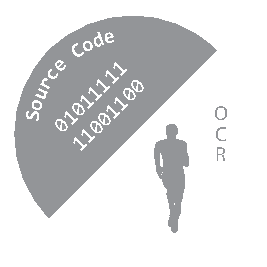
\includegraphics[width=0.6\textwidth]{Grafiken/Logo-Grau.pdf}
\caption{Logo-Grau}
\label{fig:Logo-Grau}%% anpassen
\end{figure}

Logo-negativ vgl.~(\autoref{fig:Logo-negativ}).

\begin{figure}[!hb]% hier: !hb
\centering

\includegraphics[width=0.6\textwidth]{Grafiken/Logo-negativ.pdf}
\caption{Logo-negativ}
\label{fig:Logo-negativ}%% anpassen
\end{figure}

Logo-SW vgl.~(\autoref{fig:Logo-SW}).

\begin{figure}[!hb]% hier: !hb
\centering
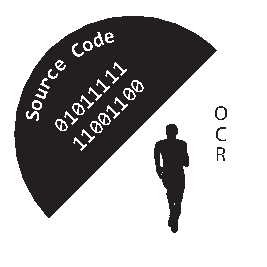
\includegraphics[width=0.6\textwidth]{Grafiken/Logo-SW.pdf}
\caption{Logo-SW}
\label{fig:Logo-SW}%% anpassen
\end{figure}


\section{KOM}\label{kom}

Tür Endschalter Hess vgl.~(\autoref{fig:Tuer-Endschalter-Hess}).

\begin{figure}[!hb]% hier: !hb
\centering
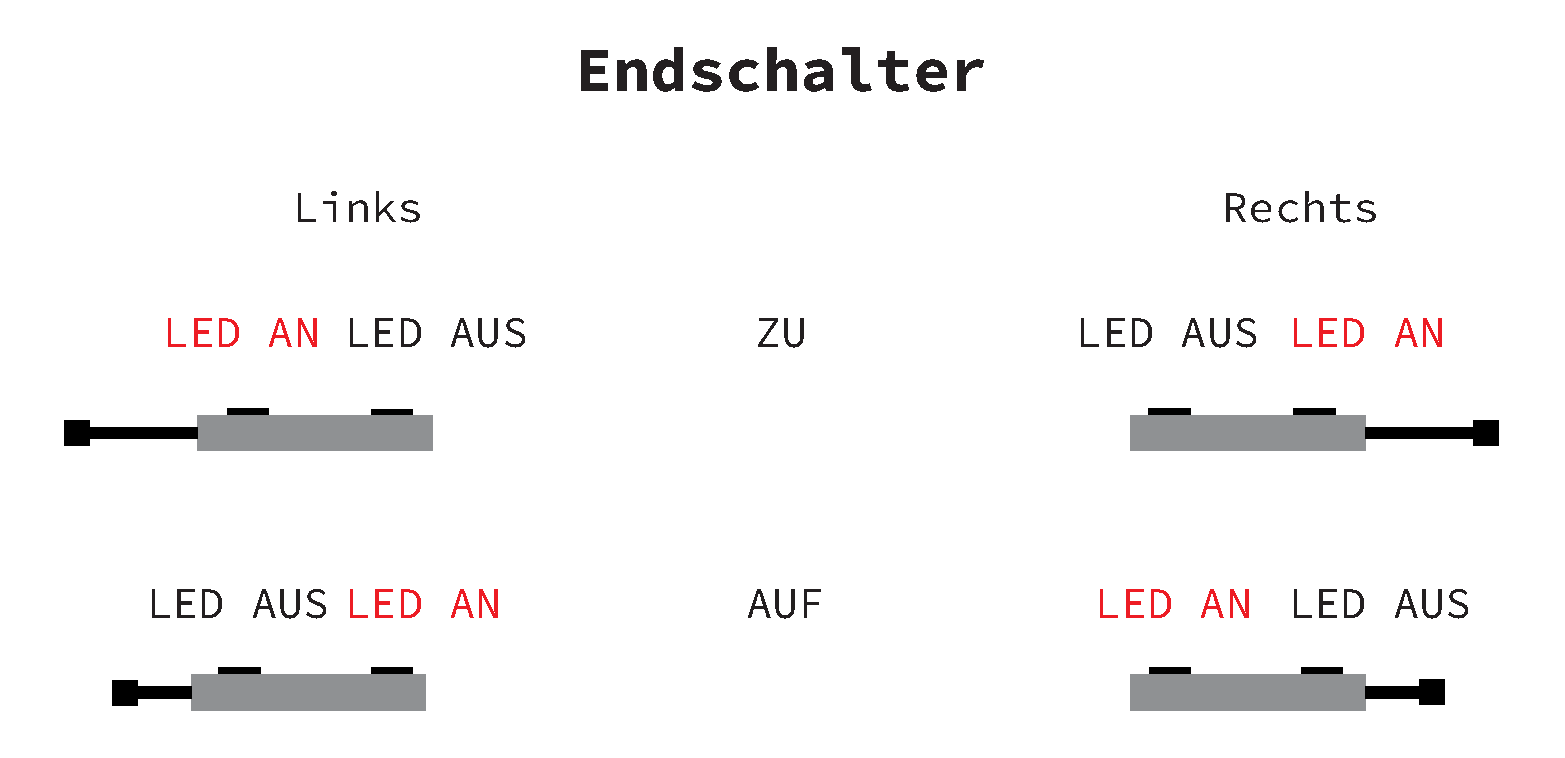
\includegraphics[width=0.6\textwidth]{Grafiken/Tuer-Endschalter-Hess.pdf}
\caption{Tür Endschalter Hess}
\label{fig:Tuer-Endschalter-Hess}%% anpassen
\end{figure}

Türlaufsensor Hess vgl.~(\autoref{fig:Tuer-Tuerlaufsensor-Hess}).

\begin{figure}[!hb]% hier: !hb
\centering
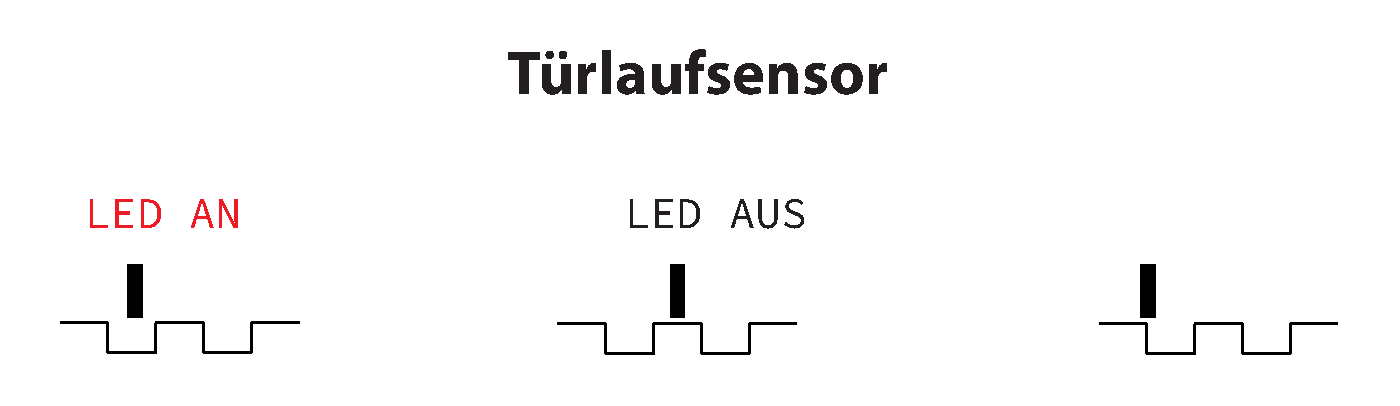
\includegraphics[width=0.6\textwidth]{Grafiken/Tuer-Tuerlaufsensor-Hess.pdf}
\caption{Türlaufsensor Hess}
\label{fig:Tuer-Tuerlaufsensor-Hess}%% anpassen
\end{figure}

\section{GIT}\label{git}

Git-Entwicklung vgl.~(\autoref{fig:Git-Entwicklung}).

\begin{figure}[!hb]% hier: !hb
\centering
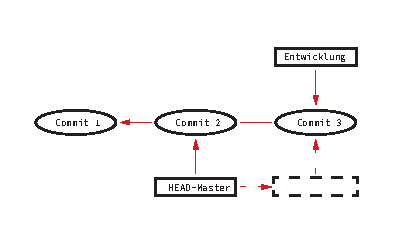
\includegraphics[width=0.6\textwidth]{Grafiken/Git-Entwicklung.pdf}
\caption{Git-Entwicklung}
\label{fig:Git-Entwicklung}%% anpassen
\end{figure}

Git-Parallel vgl.~(\autoref{fig:Git-Parallel}).

\begin{figure}[!hb]% hier: !hb
\centering
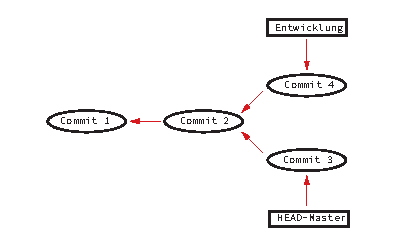
\includegraphics[width=0.6\textwidth]{Grafiken/Git-Parallel.pdf}
\caption{Git-Parallel}
\label{fig:Git-Parallel}%% anpassen
\end{figure}

Git-Team vgl.~(\autoref{fig:Git-Team}).

\begin{figure}[!hb]% hier: !hb
\centering
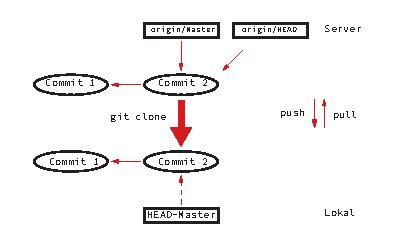
\includegraphics[width=0.6\textwidth]{Grafiken/Git-Team.pdf}
\caption{Git-Team}
\label{fig:Git-Team}%% anpassen
\end{figure}

Git-Workflow vgl.~(\autoref{fig:Git-Workflow}).

\begin{figure}[!hb]% hier: !hb
\centering
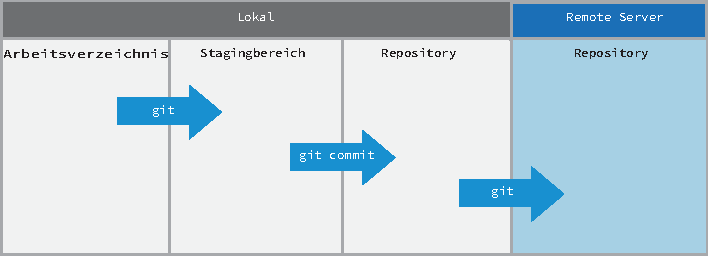
\includegraphics[width=0.6\textwidth]{Grafiken/Git-Workflow.pdf}
\caption{Git-Workflow}
\label{fig:Git-Workflow}%% anpassen
\end{figure}

Git-Wiederherstellen vgl.~(\autoref{fig:Git-Wiederherstellen}).

\begin{figure}[!hb]% hier: !hb
\centering
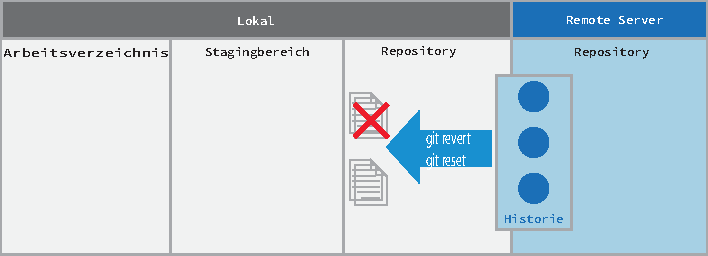
\includegraphics[width=0.6\textwidth]{Grafiken/Git-Wiederherstellen.pdf}
\caption{Git-Wiederherstellen}
\label{fig:Git-Wiederherstellen}%% anpassen
\end{figure}

Git-Reset-Revert vgl.~(\autoref{fig:Git-Reset-Revert}).

\begin{figure}[!hb]% hier: !hb
\centering
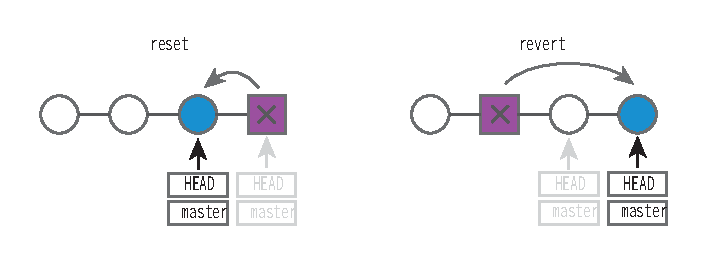
\includegraphics[width=0.6\textwidth]{Grafiken/Git-Reset-Revert.pdf}
\caption{Git-Reset-Revert}
\label{fig:Git-Reset-Revert}%% anpassen
\end{figure}

Git-Rueckgaengig vgl.~(\autoref{fig:Git-Rueckgaengig}).

\begin{figure}[!hb]% hier: !hb
\centering
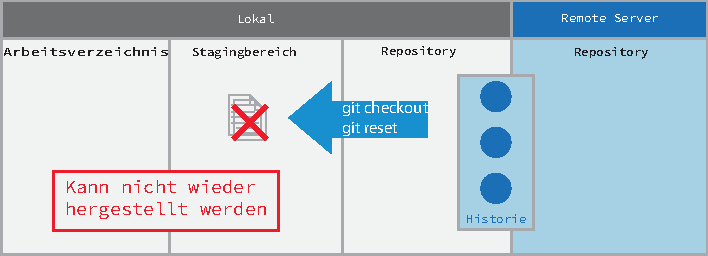
\includegraphics[width=0.6\textwidth]{Grafiken/Git-Rueckgaengig.pdf}
\caption{Git-Rueckgaengig}
\label{fig:Git-Rueckgaengig}%% anpassen
\end{figure}



\section{Backup-Plan}\label{backup-plan}

Backup-Plan vgl.~(\autoref{fig:Backup-Plan}).

\begin{figure}[!hb]% hier: !hb
\centering
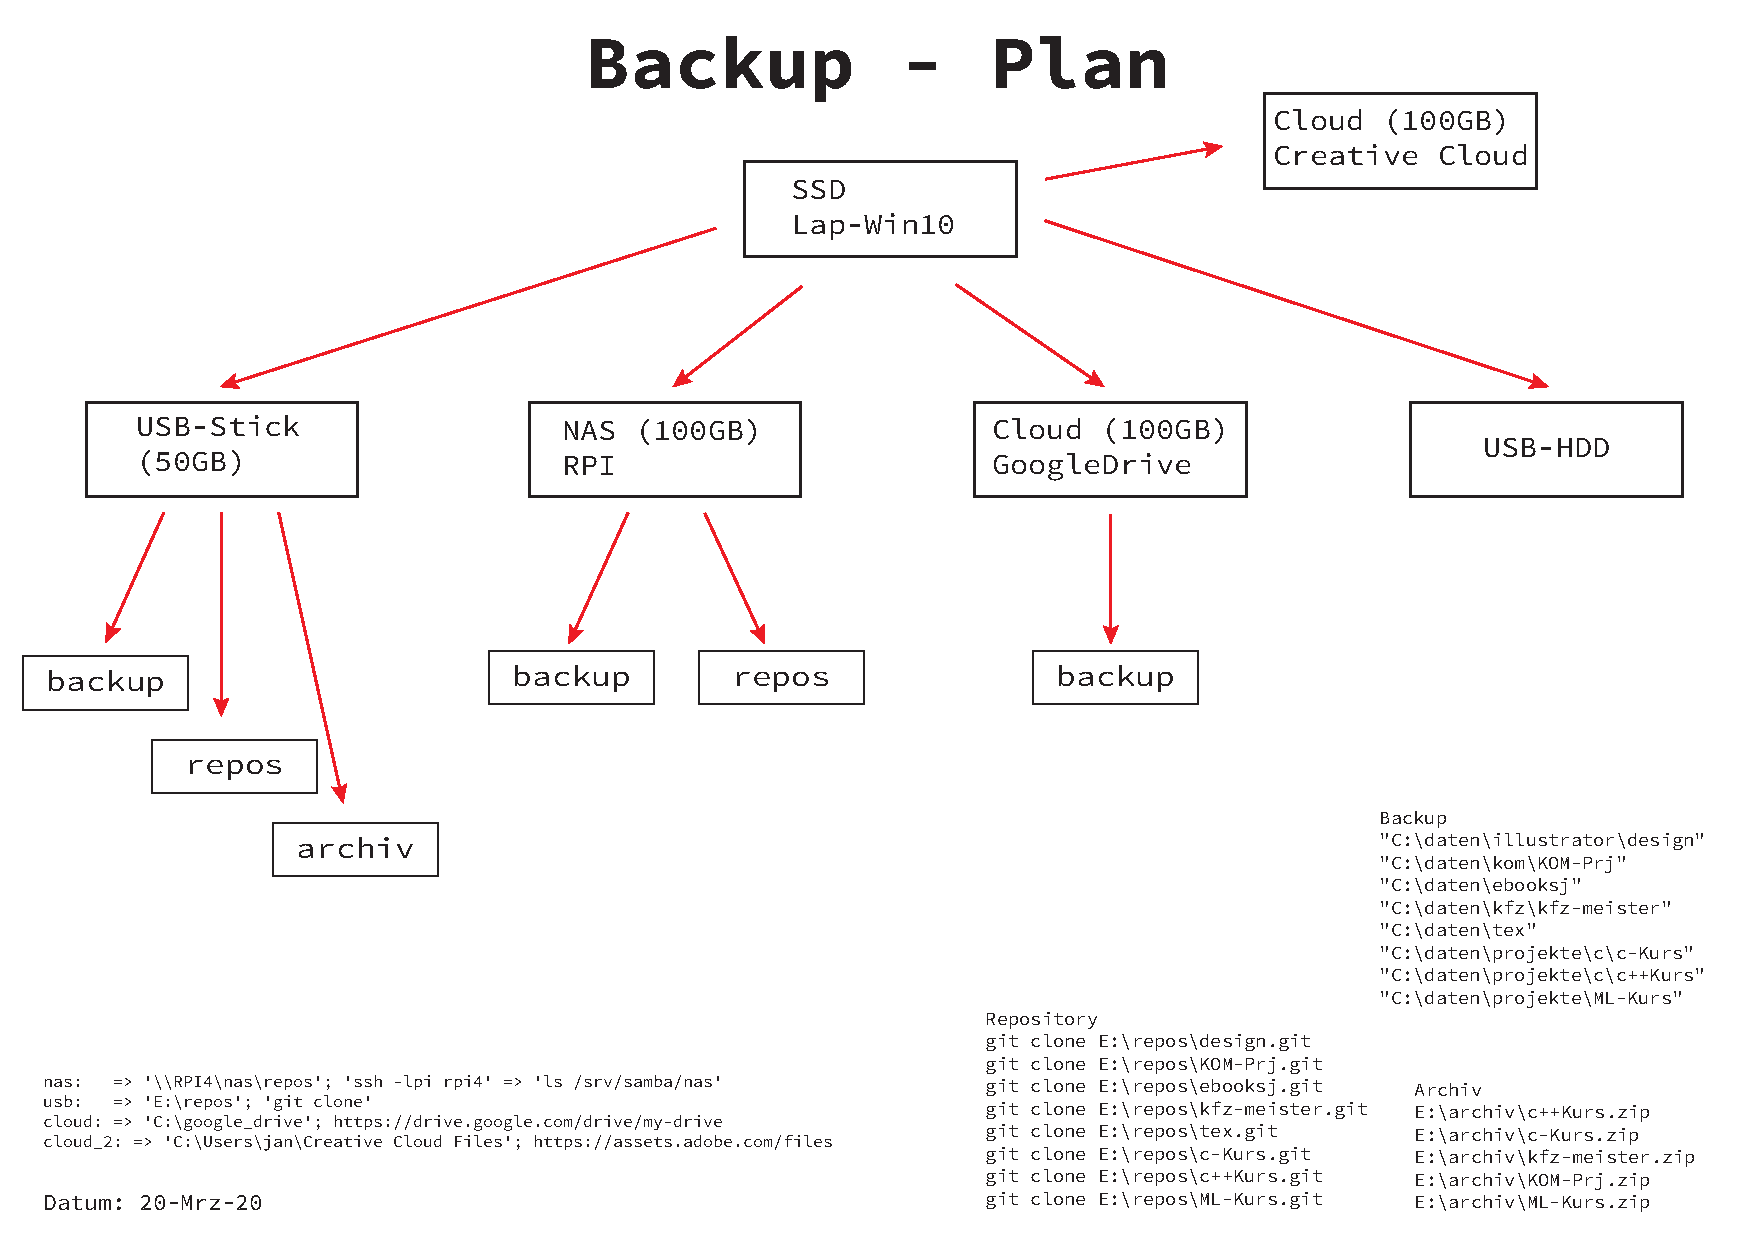
\includegraphics[width=0.6\textwidth]{Grafiken/Backup-Plan.pdf}
\caption{Backup-Plan}
\label{fig:Backup-Plan}%% anpassen
\end{figure}


\section{Form erstellen mit Illustrator}\label{}

AI-FK vgl.~(\autoref{fig:AI-FK}).

\begin{figure}[!hb]% hier: !hb
\centering

\includegraphics[width=0.6\textwidth]{Grafiken/AI-FK.pdf}
\caption{AI-FK}
\label{fig:AI-FK}%% anpassen
\end{figure}

AI-Einfache-Formen vgl.~(\autoref{fig:AI-Einfache-Formen}).

\begin{figure}[!hb]% hier: !hb
\centering

\includegraphics[width=0.6\textwidth]{Grafiken/AI-Einfache-Formen.pdf}
\caption{AI-Einfache-Formen}
\label{fig:AI-Einfache-Formen}%% anpassen
\end{figure}


AI-Form-erstellen vgl.~(\autoref{fig:AI-Form-erstellen}).

\begin{figure}[!hb]% hier: !hb
\centering
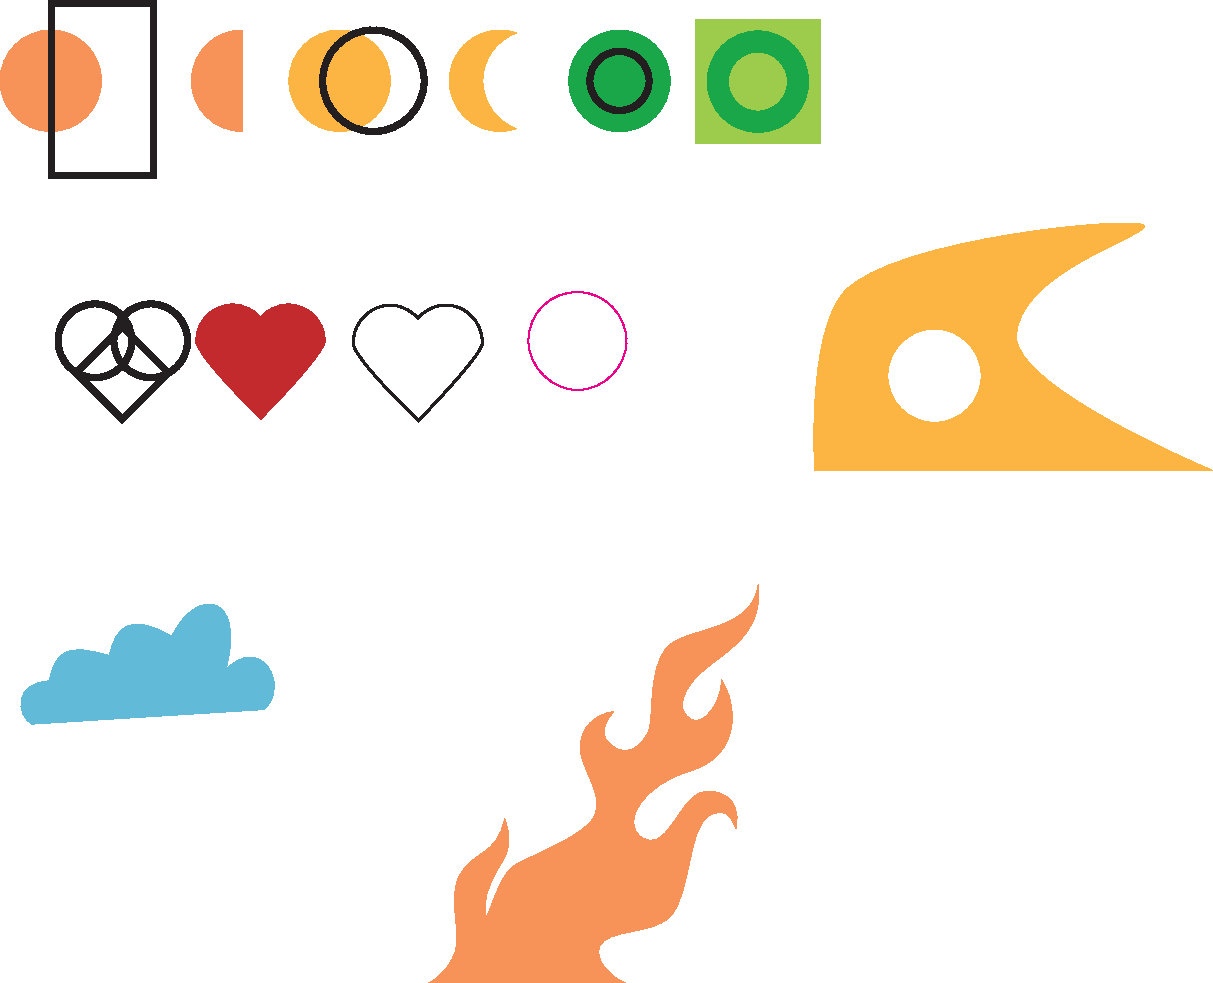
\includegraphics[width=0.6\textwidth]{Grafiken/AI-Form-erstellen.pdf}
\caption{AI-Form-erstellen}
\label{fig:AI-Form-erstellen}%% anpassen
\end{figure}

AI-PFP vgl.~(\autoref{fig:AI-PFP}).

\begin{figure}[!hb]% hier: !hb
\centering

\includegraphics[width=0.6\textwidth]{Grafiken/AI-PFP.pdf}
\caption{AI-PFP}
\label{fig:AI-PFP}%% anpassen
\end{figure}

AI-PPP vgl.~(\autoref{fig:AI-PPP}).

\begin{figure}[!hb]% hier: !hb
\centering

\includegraphics[width=0.6\textwidth]{Grafiken/AI-PPP.pdf}
\caption{AI-PPP}
\label{fig:AI-PPP}%% anpassen
\end{figure}

AI-Symmetrie vgl.~(\autoref{fig:AI-Symmetrie}).

\begin{figure}[!hb]% hier: !hb
\centering

\includegraphics[width=0.6\textwidth]{Grafiken/AI-Symmetrie.pdf}
\caption{AI-Symmetrie}
\label{fig:AI-Symmetrie}%% anpassen
\end{figure}

